%% The following is a directive for TeXShop to indicate the main file
%%!TEX root = diss.tex

\chapter{Introduction}
\label{ch:Introduction}

This first paragraph will give a little intro and describe what is coming up in \autoref{sec:Cosmology}, \autoref{sec:Lensing} and \autoref{sec:Clusters}.

%%%%%%%%%%%%%%%%%%%%%%%%%%%%%%%%%%%%%%%%%%%%%%%%%%%%%%%%%%%%%%%%%%%%%%
\section{Cosmology}
\label{sec:Cosmology}

\subsection{Our Universe}

The \acf{CFHTLenS} was a big lensing project in the \acf{CFHTLS} survey. This is an example of an acronym that does not go in the table of acronyms:  \acs{UBC}. This section is supposed to be on cosmology...

\subsection{Distances in Cosmology}

%%%%%%%%%%%%%%%%%%%%%%%%%%%%%%%%%%%%%%%%%%%%%%%%%%%%%%%%%%%%%%%%%%%%%%
\section{Galaxy Clusters}
\label{sec:Clusters}

\subsection{Clusters as Cosmological Probes}

\subsection{Intracluster Physics}

%%%%%%%%%%%%%%%%%%%%%%%%%%%%%%%%%%%%%%%%%%%%%%%%%%%%%%%%%%%%%%%%%%%%%%
\section{Gravitational Lensing}
\label{sec:Lensing}

As light from distance objects in the universe makes the journey from its source to our telescopes, it is deflected and distorted by mass inhomogeneities along its path. In particular, large overdensities, such as galaxies and galaxy clusters, will cause light rays to be bent 

\begin{figure}
\begin{center}
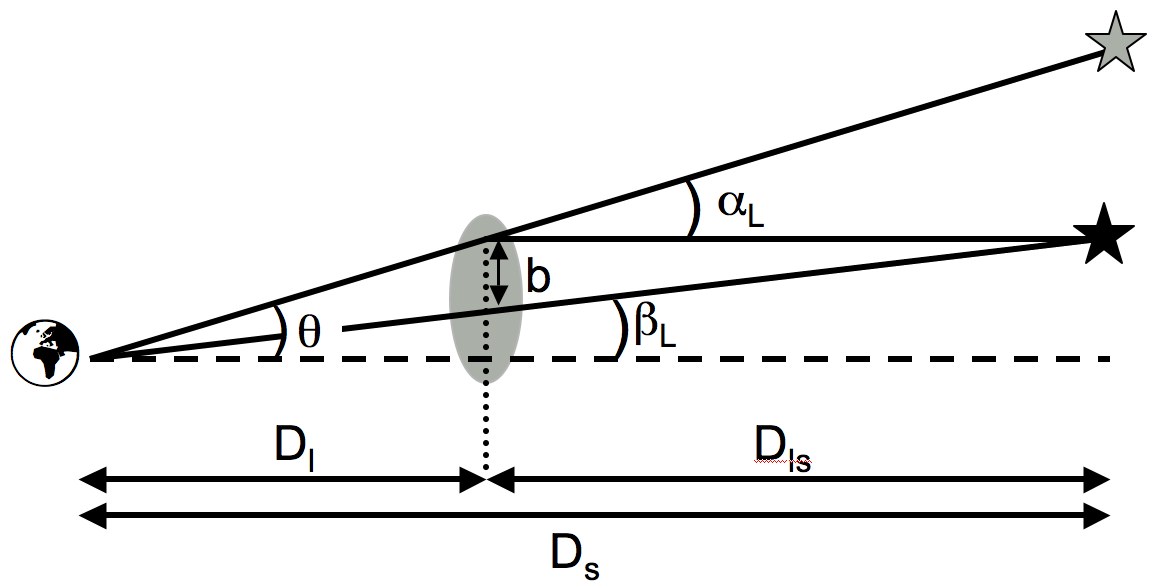
\includegraphics[scale=0.3]{plots_intro/LensDiagram.png}
\caption[Gravitational Lensing Diagram]{Diagram showing the geometry of gravitational lensing. Light from the background source is bent by an angle $\alpha$ when it passes near the gravitational lens (gray oval) on its way to the earth. While the actual source (black star) is at an angle $\beta$ relative to the horizontal, its image (gray star) appears to be at an angle $\alpha+\beta$. The angular diameter distances to the lens ($D_{\rm l}$), to the source ($D_{\rm s}$) and between the lens and source ($D_{\rm ls}$) are labelled.}
\label{lensing}
\end{center}
\end{figure}


\subsection{Weak Lensing Shear}

\subsection{Magnification}

\subsection{Magnification vs. Shear}

%%%%%%%%%%%%%%%%%%%%%%%%%%%%%%%%%%%%%%%%%%%%%%%%%%%%%%%%%%%%%%%%%%%%%%
\section{Impact of this Thesis}
\label{sec:impact}


%%%%%%%%%%%%%%%%%%%%%%%%%%%%%%%%%%%%%%%%%%%%%%%%%%%%%%%%%%%%%%%%%%%%%%
\section{Thesis Overview}
\label{sec:overview}


%%%%%%%%%%%%%%%%%%%%%%%%%%%%%%%%%%%%%%%%%%%%%%%%%%%%%%%%%%%%%%%%%%%%%%
\endinput
Any text after an \endinput is ignored.
You could put scraps here or things in progress.
